\documentclass{article}
\usepackage{graphicx} 
\usepackage{tikz}% Required for inserting images
%\usepackage[letterpaper,top=2.54cm,bottom=2.54cm,left=3.17cm,right=3.17cm,marginparwidth=1.75cm]{geometry}
\usepackage[margin=1in]{geometry}
\usepackage{hyperref}
\usepackage{setspace}
\usepackage{amsmath}
\hypersetup{
    colorlinks=true,
    linkcolor=blue,
    filecolor=magenta,      
    urlcolor=cyan,
    pdftitle={Overleaf Example},
    pdfpagemode=FullScreen,
}

\renewcommand{\includegraphics}[2][]{}

\title{Practical Concerns for Estimating Mixed Hidden Markov Models}
\author{}
\date{}

\doublespacing

\begin{document}

\maketitle

\section{Introduction}

The circadian rhythm plays a wide-ranging role in human health, from regulating important metabolomic pathways \cite{potterCircadianRhythmSleep2016} to immune response \cite{sharmaCircadianRhythmDisruption2016}. 
Disruption of the circadian rhythm is associated with a variety of negative health outcomes. 
For instance, sleep disruption related to shift work is most likely carcinogenic \cite{iarc2010}.
Polysomnography (PSG) is the gold standard when evaluating certain sleep disorders, however PSG is both costly and inconvenient for the patient\cite{chervin1999}. 
Requiring an overnight study at a specific heath care facility, there has been considerable interest in finding a cost-effective replacement.  As PSG is not readily available it is difficult to amass population level data. 

The proliferation of personal physical activity monitors (PAM) offers an interesting insight into sleep health. 
Actigraphy has proven to be useful in assessing circadian rhythm disorders \cite{morgenthaler2007} and has some distinct advantages over PSG. 
PAMs collect a large amount of data over a longer period of time. As 
they are relatively inexpensive, we can collect more data on more people compared to PSG.  
Although this is an exciting opportunity, there are challenges. Actigraphy measures movement, not sleep. We can reconstruct the sleep cycle from actigraphy data, however we cannot measure the different stages nor the subjective experience of sleep. 
In addition, constraints of wearable devices must also be considered \cite{imtiaz2021}, such as detection limit issues. 

Although there is a clear connection between activity and sleep, the specific relationship is difficult to ascertain. 
High activity periods most likely indicate an underlying wake state, however periods of inactivity may be hard to classify. 
Activity data may look similar for sedentary wake activities and sleep (e.g. watching TV may appear similar sleeping). 
During periods of very low activity, measurements may be below the limit of detection (LoD). 
We propose to use an extension of a hidden Markov model (HMM) to capture this behavior. 
The observed data will be the activity measurements from the PAM and the hidden Markov state will be the unobserved wake/sleep status.

HMM Actigraphy PARA

As physical activity is not uniform among people \cite{hootman2003}, any study utilizing population level actigraphy data must account for this. 
Previously this issue has been handled by either extending the Markov state space from wake and sleep to high activity wake, low activity wake, and sleep or by estimating the emission parameters independently for each person. 
In the first scenario, active people would spend a larger proportion of their wake time in the high activity wake state compared to the low activity wake state. 
This solution may cause more problems than it solves as there is no agreed upon cut off for what constitutes low/high activity. 
Additionally, this greatly increases the complexity of adding important covariates to the Markov transition matrix. 
Estimating a 3x3 transition matrix is much more difficult than a 2x2, causing feasibility issues when large amounts of data are used. 
For the second approach, although estimating the emission parameters independently allows a greater fit this too causes more issues than it solves. 
As the number of participants increases so too does the number of parameters. 
For datasets that do not have a large number of repeated measurements for each person this approach will not work. 
Lastly, it is not clear how this can be extrapolated to new data without re-estimation. 
Instead, we propose a mixed HMM (MHMM) \cite{Altman2007} with an individual level random effect for the activity data in the wake state. 
This allows people to have different levels of activity while keeping the interpretable and computation friendly two state structure.
We use a non-parametric approach to estimate this heterogeneity as there is little precedent on how activity is distributed across the US population and we did not want to assume any particular distribution.

The National Health Examination Survey (NHANES) is a collection of studies aiming to quantify the health of US civilians. 
Beginning in 1960, NHANES become a yearly study in 1999 where specific goals change year-to-year to focus on emerging issues. 
For two years in the mid 2010s, a representative sample for the US of 5,000 participants (for a total of 10,000) were given a wrist physical activity monitor (PAM) for 9 days. 
Among other metrics, these PAMs measured physical activity by the minute. 
This data offers a unique glimpse into the circadian rhythm for the US population as a whole.

This project focuses on practical concerns for estimation of a MHMM, with a focus on guidelines for estimating MHMMs. 
Specifically, we aim to answer whether a MHMM is necessary for state reconstruction, or if a HMM is sufficient. 
If a MHMM is necessary, we discuss how many support points are needed for the nonparametric density estimation for the emission distribution random effect (RE). 
Afterwards we apply a MHMM to the NHANES physical activity data.

\section{Methods} \label{Methods}
\subsection{Notation}

Define the set $\{S_{i1}, ..., S_{iT}\}$ as the states of a first order Markov chain (MC) corresponding to the sleep-wake cycle. If person $i$ at time $t$ is awake then $S_{it}=0$, if person $i$ is asleep at time $t$ then $S_{it}=1$. To account for detection limit issues, let $\delta_{it}$ be 0 when the activity measurement is below the LoD at time $t$ and person $i$ is asleep, and 1 otherwise. We assume that when we observe a measurement below the LoD, the person must be in the sleep state. This first order MC can be completely described by an initial probability, $P_j=P(S_{i1} =j)$, and a (possibly non-homogenous) transition array where entry $kj$ is equal to $P_{kj}(it)=P(S_{it}=j|S_{it-1}=k)$. Define the set $\{a_{i1}, ..., a_{iT}\}$ as the observed physical activity data from a PAM for patient $i$. For person $i$ at time t, we refer to the distribution of the activity measurement given the current wake/sleep state as the emission distribution. $a_{it}$ given the current sleep status is independent of all other MC states, or equivalently $P(a_{it}|S_{i1}, ..., S_{iT}) = P(a_{it}|S_{it})$. Therefore, the HMM can be completely described by the initial, transition, and emission probabilities.

To allow for covariates in the transition probabilities, we model the probability of changing states with the expit function. We have $P_{01}(it) = \text{expit}(X_{it}\beta_0)$ and $P_{10}(it) = \text{expit}(X_{it}\beta_1)$ where $X_{it}$ is a vector of covariates and $\beta_j$ is the corresponding vector of covariate parameters. This allows both fixed (e.g. race) and time-varying (e.g. current time) covariates to influence the transition probabilities.

We assume that the emission distribution is the normal distribution. When person $i$ is asleep, we assume $a_{it}$ is drawn from a normal distribution centered at $\mu_1$ with variance $\sigma_1^2$. When person $i$ is awake, we assume $a_{it}$ is drawn from a normal distribution centered at $\mu_0+u_i$ with variance $\sigma_0^2$. $u_i$ is a random effect directly related to the mean wake activity of person i. In addition, the distribution for $u_i$, call it H, has mean 0, but otherwise we impose no additional restrictions. This assumption can be relaxed, however it facilitates easy comparison between simulations. We refer to the HMM with a RE in the emission distribution as a mixed HMM (MHMM).


\subsection{Estimation}

Without applying any additional techniques, the likelihood is written as equation \ref{like1}. Inside the square brackets, we evolve through the Markov chain for person i, multiplying the initial, transition, and emission probabilities. As we do not know the underlying MC state, it is not clear yet how to calculate these probabilities as the wake/sleep states are not observed. As $u_i$ is a continuous individual level random effect, we must integrate over its support for each individual. This integral is complex and requires numerical methods to solve. The next two subsections will detail how to calculate this likelihood. 

\begin{equation}\label{like1}
f(\textbf{a}|\theta) = \prod_{i=1}^n \int_U \sum_{{s_1}\cdots{s_T}} \biggr[ 
    P(S_{i1}=s_1)\prod_{t=2}^T P(S_{it}=s_t|S_{it-1}=s_{t-1}) \times 
    \prod_{t=1}^T P(a_{it}|S_{it}=s_t,u_i)^{\delta_{it}} \biggr] dH(u_i)
\end{equation}

\subsubsection{Nonparametric Density Estimation (NPDE)}

To simplify the integral (as well as allowing future computations with the forward-backward algorithm), we will estimate the continuous RE distribution, H, with a discrete random variable, $b_i$. A small number of support points are chosen where the mass put on support point l is $\pi_l$. This can equivalently be written as $P(b_i = r_l) = \pi_l$ where $r_l$ is support point l. Conceptually, this can be thought of as estimating a discrete distribution using a histogram where each bar of the histogram is a support point and the mass put on each support point is the height of the bar. Using one support point is equivalent to leaving out the RE and thus the MHMM reduces to a HMM with shared emission parameters. Using NPDE we can write the likelihood as follows: 

\begin{equation}\label{like2}
f(\textbf{a}|\theta) = \prod_{i=1}^n \sum_{l=1}^L \sum_{{s_1}\cdots{s_T}} \biggr[ 
    P(S_{i1}=s_1)\prod_{t=2}^T P(S_{it}=s_t|S_{it-1}=s_{t-1}) \times 
    \prod_{t=1}^T P(a_{it}|S_{it}=s_t,b_i=r_l)^{\delta_{it}} \biggr] \pi_l,
\end{equation}
where the integral over the support of U from equation \ref{like1} becomes a sum over the number of support points, L, in equation \ref{like2}. Thus, the time needed to compute this likelihood scales linearly with L. Increasing L increases estimation accuracy, however it comes at a computational price. L must be chosen before estimation, and there are no clear guidelines on how to do so. Following a simulation study in section \ref{SimStudy}, we will discuss how to choose the number of support points.

\subsubsection{EM Algorithm}

The EM algorithm is an iterative technique to preform maximum likelihood estimation in the presence of latent variables \cite{Baum1970}. Each iteration of the algorithm alternates between an expectation (E) and maximization (M) step, where the likelihood increases each iteration. Once this increase becomes sufficiently small, we consider the algorithm converged and stop. For the E step, we calculate the expected value of the full data log likelihood conditional on the observed data. We then maximize this expectation in the M step. The complete data likelihood, written down as if we knew the latent variables that are required for estimation, is: 

\begin{equation}\label{cdata}
\begin{split}
    f(\textbf{a},\textbf{S}, \textbf{b} | \theta)  = & \prod_{i=1}^n \prod_{j=0}^1 
        P(S_{i1}=j)^{I(S_{i1}=j)} \times \\
    & \prod_{i=1}^n \prod^T_{t=2} \prod_{k=0}^1 \prod_{j=0}^1  
        P(S_{it}=j|S_{it-1}=k)^{I(S_{it-1}=k,S_{t}=j)} \times \\ 
    & \prod_{i=1}^n\prod_{l=1}^L \prod^T_{t=1}\prod_{j=0}^1 
        P(a_{it}|S_{it}=j,b_i=r_l)^{I(S_{it}=j,b_i=r_l)\delta_{it}}\\
    & \prod_{i=1}^n\prod_{l=1}^L \pi_l^{I(b_i=r_l)},
\end{split}
\end{equation}
where I() is an indicator variable equal to 1 of the inside expression is true and 0 otherwise. We then take the expected value of the log of equation \ref{cdata}, conditioning on the observed data. The result is the expectation of the complete data log likelihood. We can calculate the E step by calculating equation \ref{ecdata} using a modified version of the forward-backward algorithm, detailed in the next section.

\begin{equation}\label{ecdata}
\begin{split}
    \ell = E\big[\text{log f}(\textbf{a},\textbf{S}, \textbf{b} | \theta) | \textbf{a},\theta\big]  = 
        & \sum_{i=1}^n\sum_{j=0}^1P(S_{i1}=j|\textbf{a})\text{log }P_j + \\
    & \sum_{i=1}^n \sum^T_{t=2} \sum_{k=0}^1 \sum_{j=0}^1 
        P(S_{it-1}=k,S_{it}=j|\textbf{a})\text{log }P_{kj}(it) + \\ 
    & \sum_{i=1}^n \sum_{l=1}^L \sum^T_{t=1}\sum_{j=0}^1 
        P(S_{it}=j,b_i=r_l|\textbf{a}) \delta_{it}\text{log}P(a_{t}|S_{it}=j, b_i=r_l) + \\
    &  \sum_{i=1}^n \sum_{l=1}^L P(b_i=r_l|\textbf{a}) \text{log }\pi_l 
\end{split}
\end{equation}

\subsubsection{Forward-backward Algorithm}
To account for the random effect in the emission distribution we use a modified version of the forward-backward algorithm that conditions on the discrete RE for person $i$ \cite{Maruotti2011}. The forward and backward quantities are $\alpha_{it}(j,r_l) = P(a_{i1}, ..., a_{it}, S_{it} = j | b_i=r_l)$ and $\beta_{it}(j,r_l) =  P(a_{it+1}, ..., a_{iT} | S_{it} = j,b_i=r_l)$, respectively. Equations \ref{fwd} and \ref{bkwd} detail the recursive calculations. Equations \ref{proba}-\ref{probstran} can then be calculated, which are necessary for the M step.  
 
\begin{equation} \label{fwd}
\alpha_{it}(j,r_l) = \begin{cases}
    p_{j} f(a_{i1}|S_{i1}=j,r_l) & \text{if } t = 1 \\
    \sum_{k=0}^1 \alpha_{it-1} (k,b_l)p_{kj}P(a_{it}|S_{it}=j,b_i=r_l)^{\delta_{it}} 
        & \text{if } t > 1\\
\end{cases}
\end{equation}

\begin{equation} \label{bkwd}
\beta_{it}(j,r_l) = \begin{cases} 
    \sum_{k=0}^1p_{jk}P(a_{it+1}|S_{it+1}=k,b_i=r_l)^{\delta_{it}}\beta_{it+1}(k,r_l) 
        & \text{if } t < n \\
    1 & \text{if } t = n \\
\end{cases}
\end{equation}


\begin{equation}\label{proba}
\begin{split}
    P(\textbf{a}) & = \prod_{i=1}^n \sum_{l=1}^L 
        P(\textbf{a}|b_{i}=r_l)P(b_{i}=r_l) = 
    \prod_{i=1}^n \sum_{l=1}^L \sum_{j=0}^1 \alpha_{iT}(j,r_l)\pi_l 
\end{split}
\end{equation}

\begin{equation}\label{probl}
\begin{split}
    P(b_{i}=r_l|\textbf{a}) & = \frac{P(\textbf{a}|b_{i}=r_l)P(b_{i}=r_l)}{P(\textbf{a})} = 
    \frac{\sum_{j=0}^1 \alpha_{iT}(j,r_l)\pi_l }{P(\textbf{a})}  
\end{split}
\end{equation}

\begin{equation}\label{probs0}
\begin{split}
    P(S_{it}=0,b_{i}=r_l|\textbf{a}) = \frac{P(S_{it}=0,\textbf{a}|b_{i}=r_l)
        P(b_{i}=r_l)}{P(\textbf{a})} = 
    \frac{\alpha_{it}(0,r_l)\beta_{it}(0,r_l)\pi_l }{P(\textbf{a})} 
\end{split}
\end{equation}

\begin{equation}\label{probs1}
\begin{split}
    P(S_{it}=1|\textbf{a}) = 
    \frac{\sum^L_{l=1}P(S_{it}=1,\textbf{a}|b_{i}=r_l)
        P(b_{i}=r_l)}{P(\textbf{a})} = 
    \frac{\sum^L_{l=1}\alpha_{it}(1,r_l)\beta_{it}(1,r_l)\pi_l }{P(\textbf{a})} 
\end{split}
\end{equation}


\begin{equation}\label{probstran}
\begin{split}
    P(S_{it-1}=k,S_{it}=j|\textbf{a}) & = 
        \frac{P(S_{it-1}=k,S_{it}=j,\textbf{a})}{P(\textbf{a})} \\
    & = \frac{\sum^L_{l=1}\alpha_{it}(k,r_l) p_{kj} P(a_{it}|S_{it}=j, b_i=r_l)
        \beta_{it}(j,r_l)\pi_l }{P(\textbf{a})} 
\end{split}
\end{equation}



\subsubsection{Parameter Estimates}

 To maximize each parameter, we set the derivative of the likelihood with respect to that parameter to 0 and solve. This approach has a modular nature as the initial, transition, emission, and mixing ($\pi_l$) probabilities can be maximized independently. Using the previously described adapted forward-backward algorithm, we can calculate equations closed form solutions for the initial, emission, and mixing parameters (equations \ref{init}-\ref{pi}). As we cannot observe $\mu_0$ or $r_l$ individually, we cannot estimate either independently. This does not pose an issue as the sum of the two quantities is the necessary component for the model and can be estimated. We will refer to $\nu_l$ as the cluster mean in future sections. 

\begin{equation}\label{init}
    \hat{p_j}  = \frac{\sum^n_{i=0} P(S_{i1}=0|\textbf{a})}{n}
\end{equation} 

\begin{equation}\label{mu0}
    \hat{\mu_0} + \hat{r_l} = \hat{\nu_l} = 
    \frac{\sum_{i=1}^n \sum_{t=1}^T a_{it}P(S_{it}=0,b_{i}=r_l|\textbf{a})}
    {\sum_{i=1}^n \sum_{t=1}^T P(S_{it}=0,b_{i}=r_l|\textbf{a})}
\end{equation} 

\begin{equation}\label{sig0}
    \hat{\sigma}_0^2 = 
    \frac{\sum_{i=1}^n \sum_{l=1}^L \sum_{t=1}^T 
        (a_{it}-\nu_l)^2 P(S_{it}=0,b_{i}=r_l|\textbf{a})}
        {\sum_{i=1}^n \sum_{l=1}^L \sum_{t=1}^T P(S_{it}=0,b_{i}=r_l|\textbf{a})}
\end{equation} 

\begin{equation}\label{mu1}
    \hat{\mu_1} = 
    \frac{\sum_{i=1}^n \sum_{t=1}^T a_{it}\delta_{it}P(S_{it}=1|\textbf{a})}
        {\sum_{i=1}^n \sum_{t=1}^T \delta_{it}P(S_{it}=1|\textbf{a})}
\end{equation} 

\begin{equation}\label{sig1}
    \hat{\sigma}_1^2 = 
    \frac{\sum_{i=1}^n \sum_{l=1}^L \sum_{t=1}^T 
        (a_{it}-\mu_1)^2 P(S_{it}=1|\textbf{a})}
        {\sum_{i=1}^n \sum_{l=1}^L \sum_{t=1}^T P(S_{it}=1|\textbf{a})}
\end{equation} 

\begin{equation}\label{pi}
    \hat{\pi_l} = \sum_{i = 1}^n \frac{P(b_i = r_l)}{n}
\end{equation}


Unlike the previous parameters, no closed form solution exists for the transition probabilities. Instead, we preform a single Newton-Raphson step at each iteration of the EM algorithm. Thus, $\beta_{j}^* = \beta_{j} - (\frac{\partial^2\ell}{\partial \beta_{j}^2})^{-1} \frac{\partial\ell}{\partial \beta_{j}}$, where $\beta_{j}$ is our current estimate and $\beta_{j}^*$ is our updated estimate. 

\newpage

\section{Simulation Study}\label{SimStudy}

\subsection{Results}\label{SimStudyResults}

As noted previously, there are no set of best practices for MHMM estimation. We conceived of this simulation study to test the following two questions. Do MHMMs provide enough of an advantage to motivate their use compared to standard HMMs? When estimating a MHMM how many support points are necessary for the NPDE of the RE distribution? Standard HMMs are often faster and easier to implement, however MHMMs may provide higher accuracy given a sufficient number of support points are used.

To determine the situations where a MHMM outperforms a standard HMM, we tested three different types of HMMs: standard HMM where each person has their own wake mean and variance activity parameter (individual HMM), standard HMM where there is a shared wake mean and variance activity parameter (shared HMM), and seven MHMMs with two to eight support points as described by section \ref{Methods}. The shared HMM is a special case of a MHMM with one support point. 

For the simulation study, we first simulate the sequence of MC states corresponding to the wake/sleep state of person $i$ at time $t$ according to pre-specified initial and transition probabilities. For transition probabilities, we let $\beta_j = \{\beta_{j0}, ..., \beta_{j4}\}$ and $X_{it} = \{1, x_{it1}, ..., x_{it4}\}$, where $x_{it1}$ and $x_{it2}$ are fixed covariates equal to 1 if that covariate applies to person i. $x_{it3} = \text{cos}(\frac{2\pi t}{96})$ and $x_{it4} = \text{sin}(\frac{2\pi t}{96})$ vary by time to account for the cyclical nature of the circadian rhythm.  Any first order harmonic function with a period of 96 can be estimated. A period of 96 was chosen as this is equivalent to dividing one day into 15 minute intervals. We vary both the number of people (1000 and 5000) and the length observations per person (one day and one week of follow up). For each person, we draw a continuous individual level RE from H. We considered different underlying RE distribution such that H is normal, gamma, normal/gamma mixture, and t with 2 degrees of freedom (figure \ref{REdist}). We then simulate the observed activity data where $a_{it} \sim N(2+u_i,1)$ if $S_{it}=0$ and $a_{it} \sim N(0,2)$ if $S_{it}=1$ and estimate the model parameters. Lastly, we use the Viterbi algorithm to construct the most likely sequence of the latent wake/sleep states given our estimated parameters. We compare the estimated sequence with the true wake/sleep sequence. This was repeated 100 times for each combination (model, number of people, length of observation, choice of H).

\begin{figure}
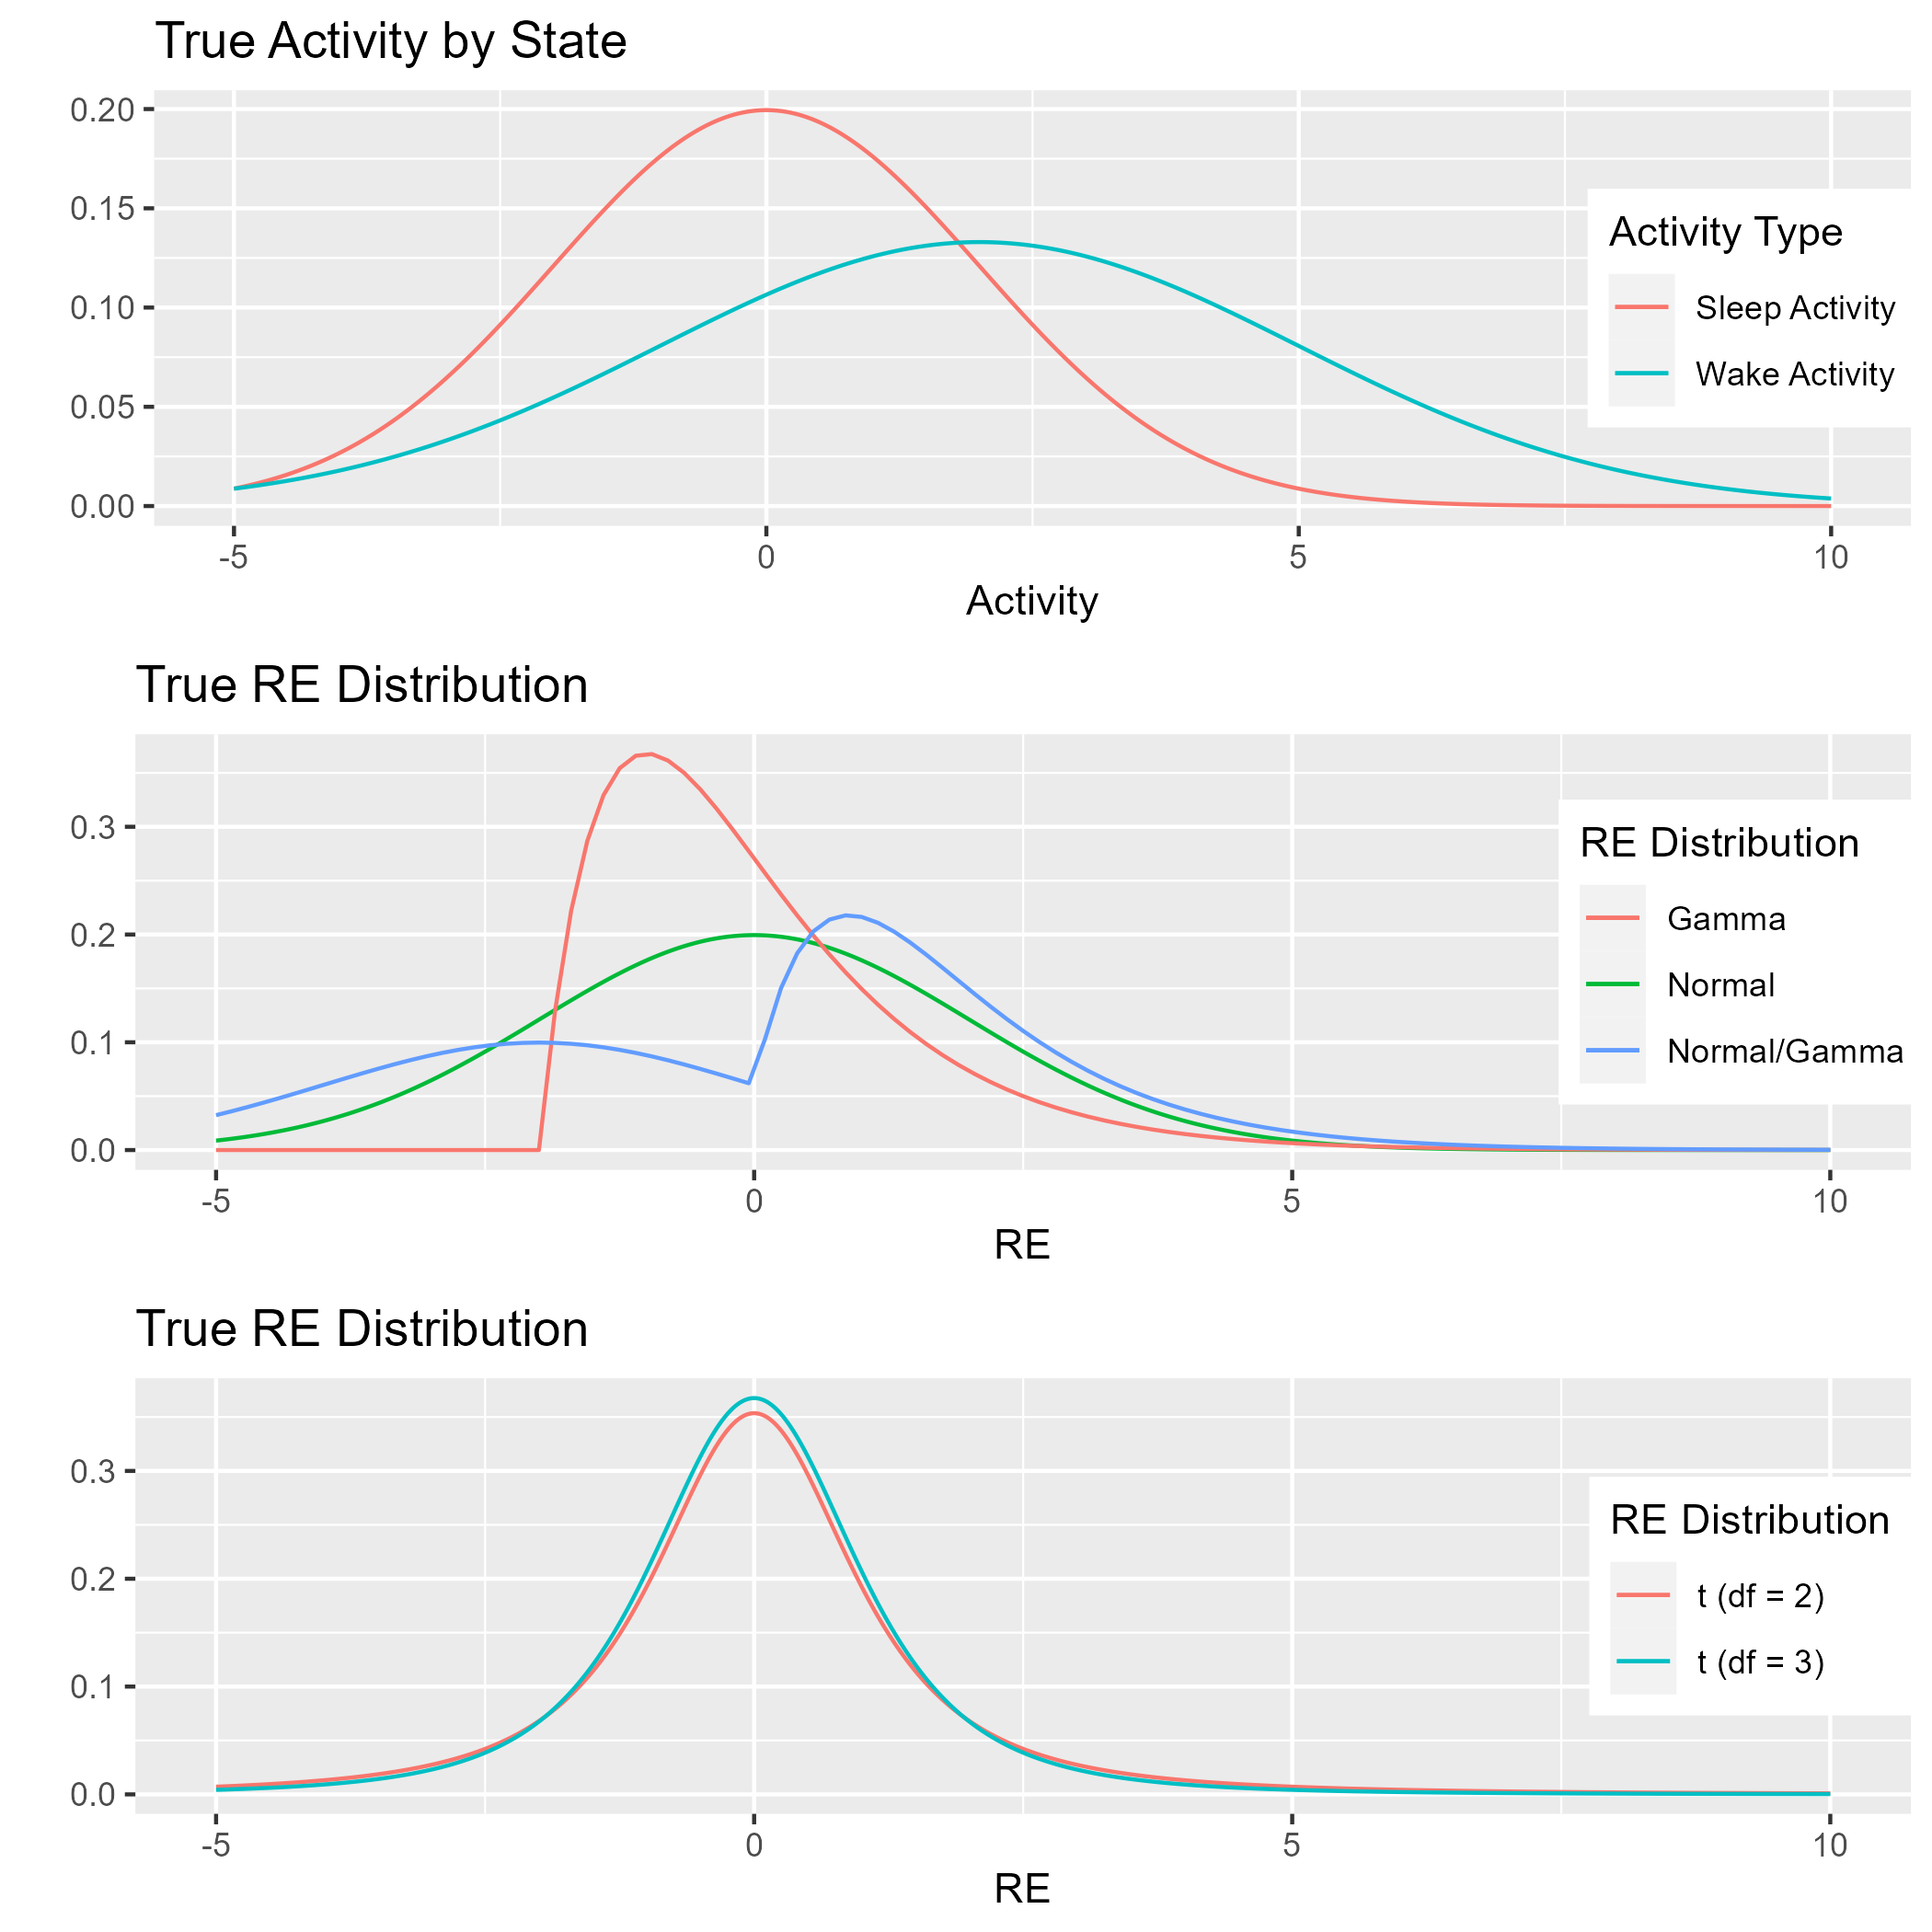
\includegraphics[scale=.5]{Support/REdist.png}
\centering
\caption{Distributions used in simulation study. Top plot shows wake 
(no RE) and sleep activity distribution. The bottom two plots show the 
different continuous RE distributions. RE distributions have been split 
up over two plots to increase readability.}
\label{REdist}
\end{figure}

The top plot of figure \ref{REdist} shows the wake (without a RE) and sleep activity distribution. Each individual's wake activity distribution would be shifted to the right or left depending on $u_i$. The bottom plot shows the different choices for H.


Figure \ref{NLacc} shows the results from the simulation in a nested loop (NL) plot. The y-axis for this figure is the accuracy of the estimated wake/sleep sequence using the true wake sleep sequence as a baseline. The color represents the model. The x-axis represents the different simulation settings (days of follow up, number of participants, and RE distribution). To read the NL plot, take for example the left most light green point. Following the gray line down, notice that point corresponds to simulated data with 1 day of follow up, 1000 participants, and H is a Gamma distribution.

As can be seen from figure \ref{NLacc}, across all simulations the shared HMM and two support point MHMM have the lowest and second-lowest accuracy, respectively. Increasing the number of support points increases the accuracy where a MHMM with 8 support points is the most accurate across all simulations. The individual HMM preforms well, with an accuracy similar to a 5 or 8 support point MHMM, depending on H and the number of observations per person. We see substantial accuracy gains from using a MHMM compared to the shared HMM when there truly is a RE in the emission distribution. We see that this accuracy increase is true for all simulation settings, meaning that the MHMM is more accurate than the shared HMM for all combinations of sample size and underlying RE distribution. The increase in accuracy from each added support point diminishes, where H determines the optimal number of support points.  

TALK MORE ABOUT IND HMM
 

\begin{figure}
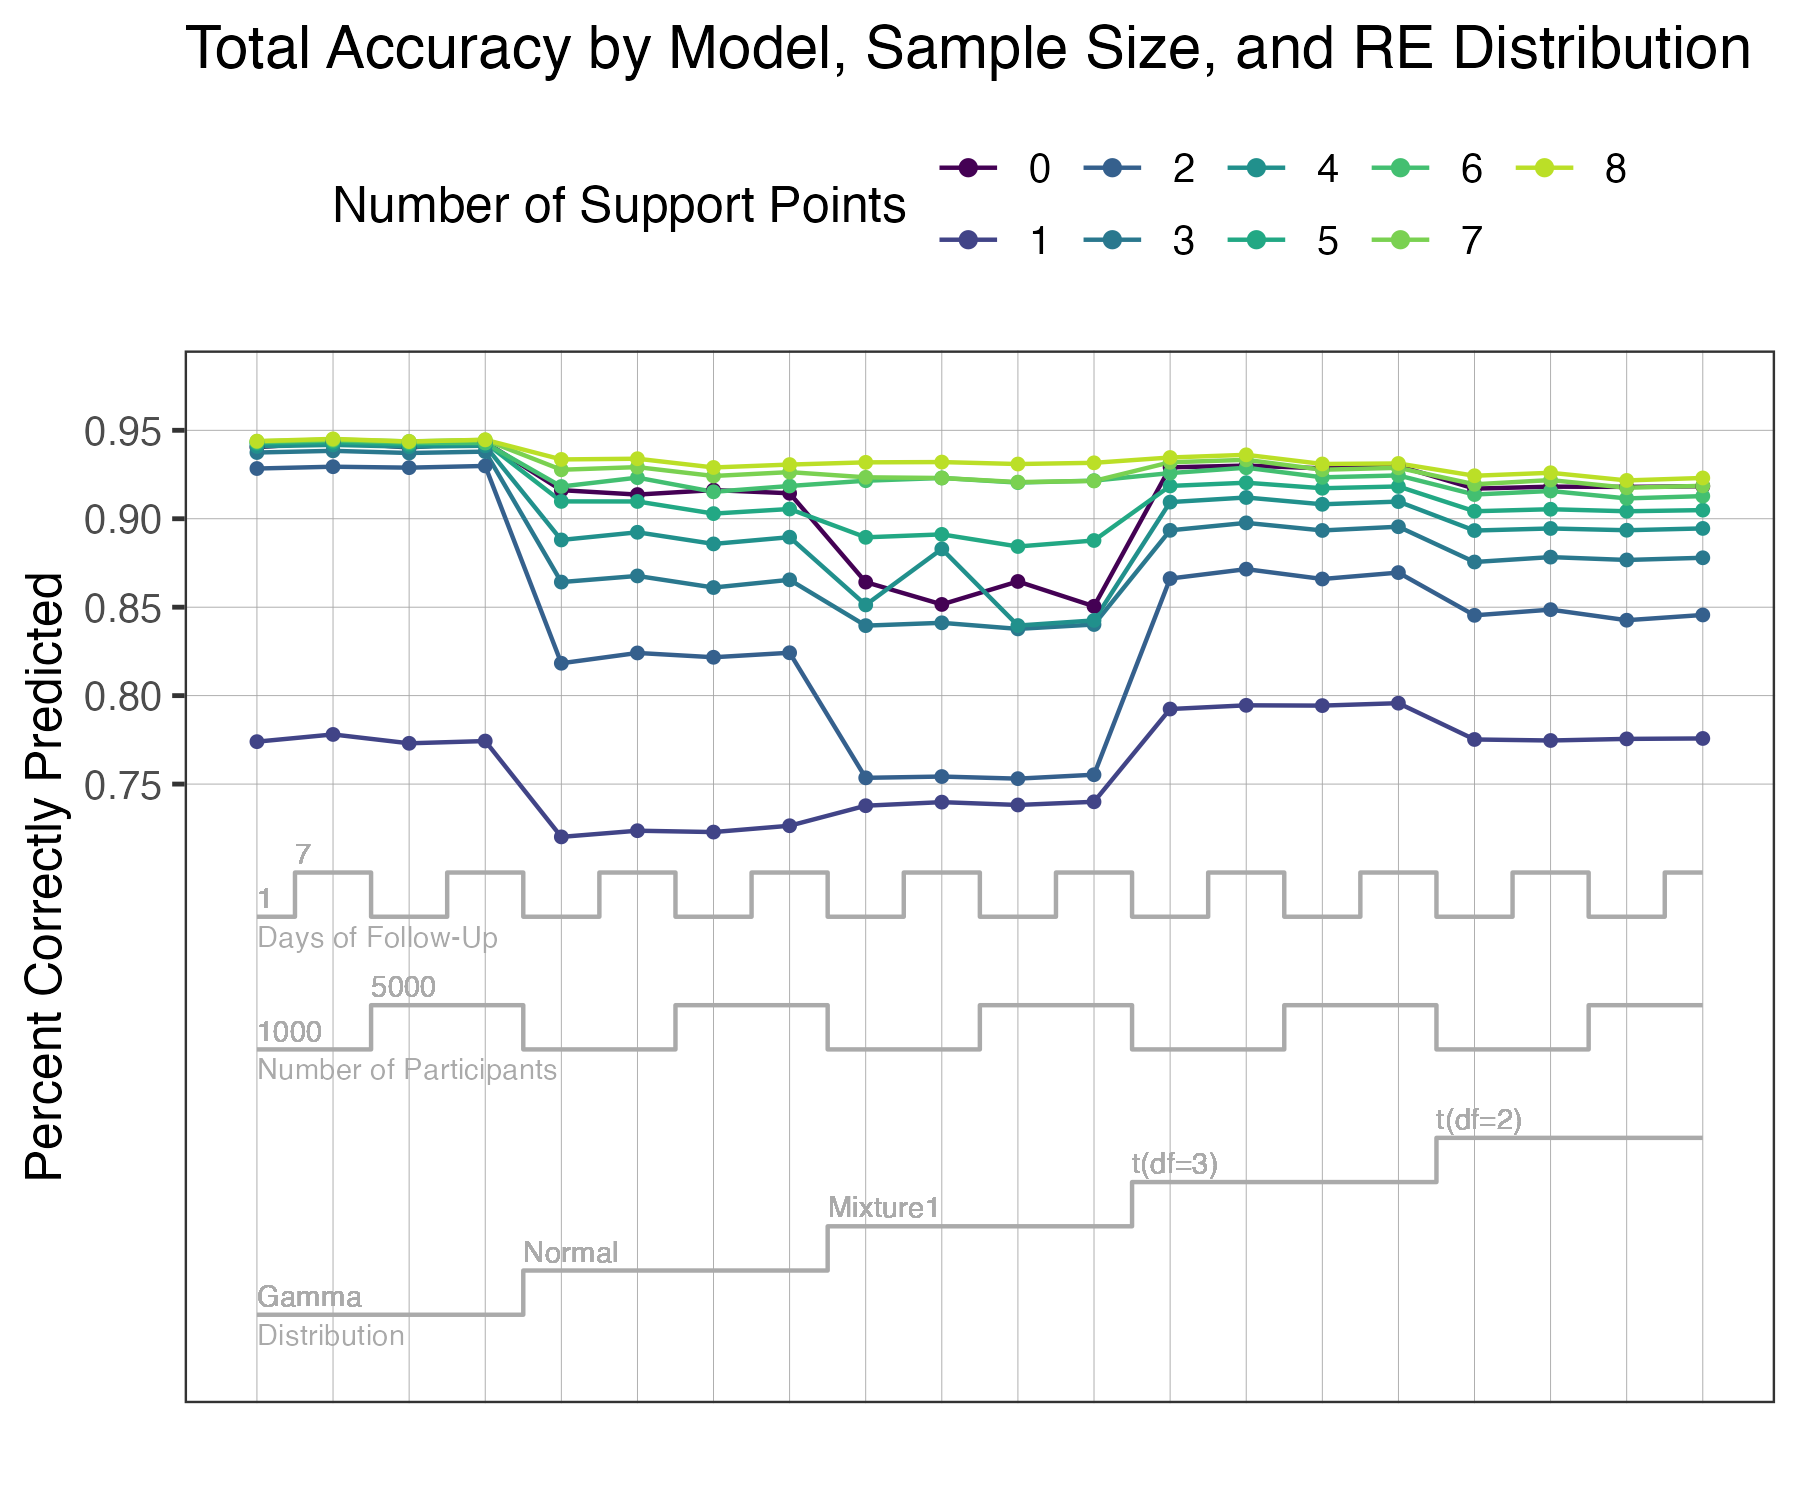
\includegraphics[scale=.8]{Support/NestedLoopAcc.png}
\centering
\caption{Nested loop plot of simulation results for total accuracy of predicted wake/sleep sequence. Each point is the median of 100 simulations and color indicates the number of support points. The X axis indicates the simulation settings, which are a combination of days follow-up, number of participants, and RE distribution.}
\label{NLacc}
\end{figure}

Now, we turn to the necessary number of support points needed for the NPDE of the RE. This is mainly dependent upon the underlying continuous RE distribution and not the sample size. There is a large increase in accuracy when the number of support points is increased from 1 (equivalent to the shared HMM) to 2, with diminishing accuracy increases afterwards. For example, when H is the Gamma distribution, there is little difference in accuracy between five and eight support points. Accuracy must be balanced with computational time as increasing the number of support points increases the running time. 


\begin{figure}
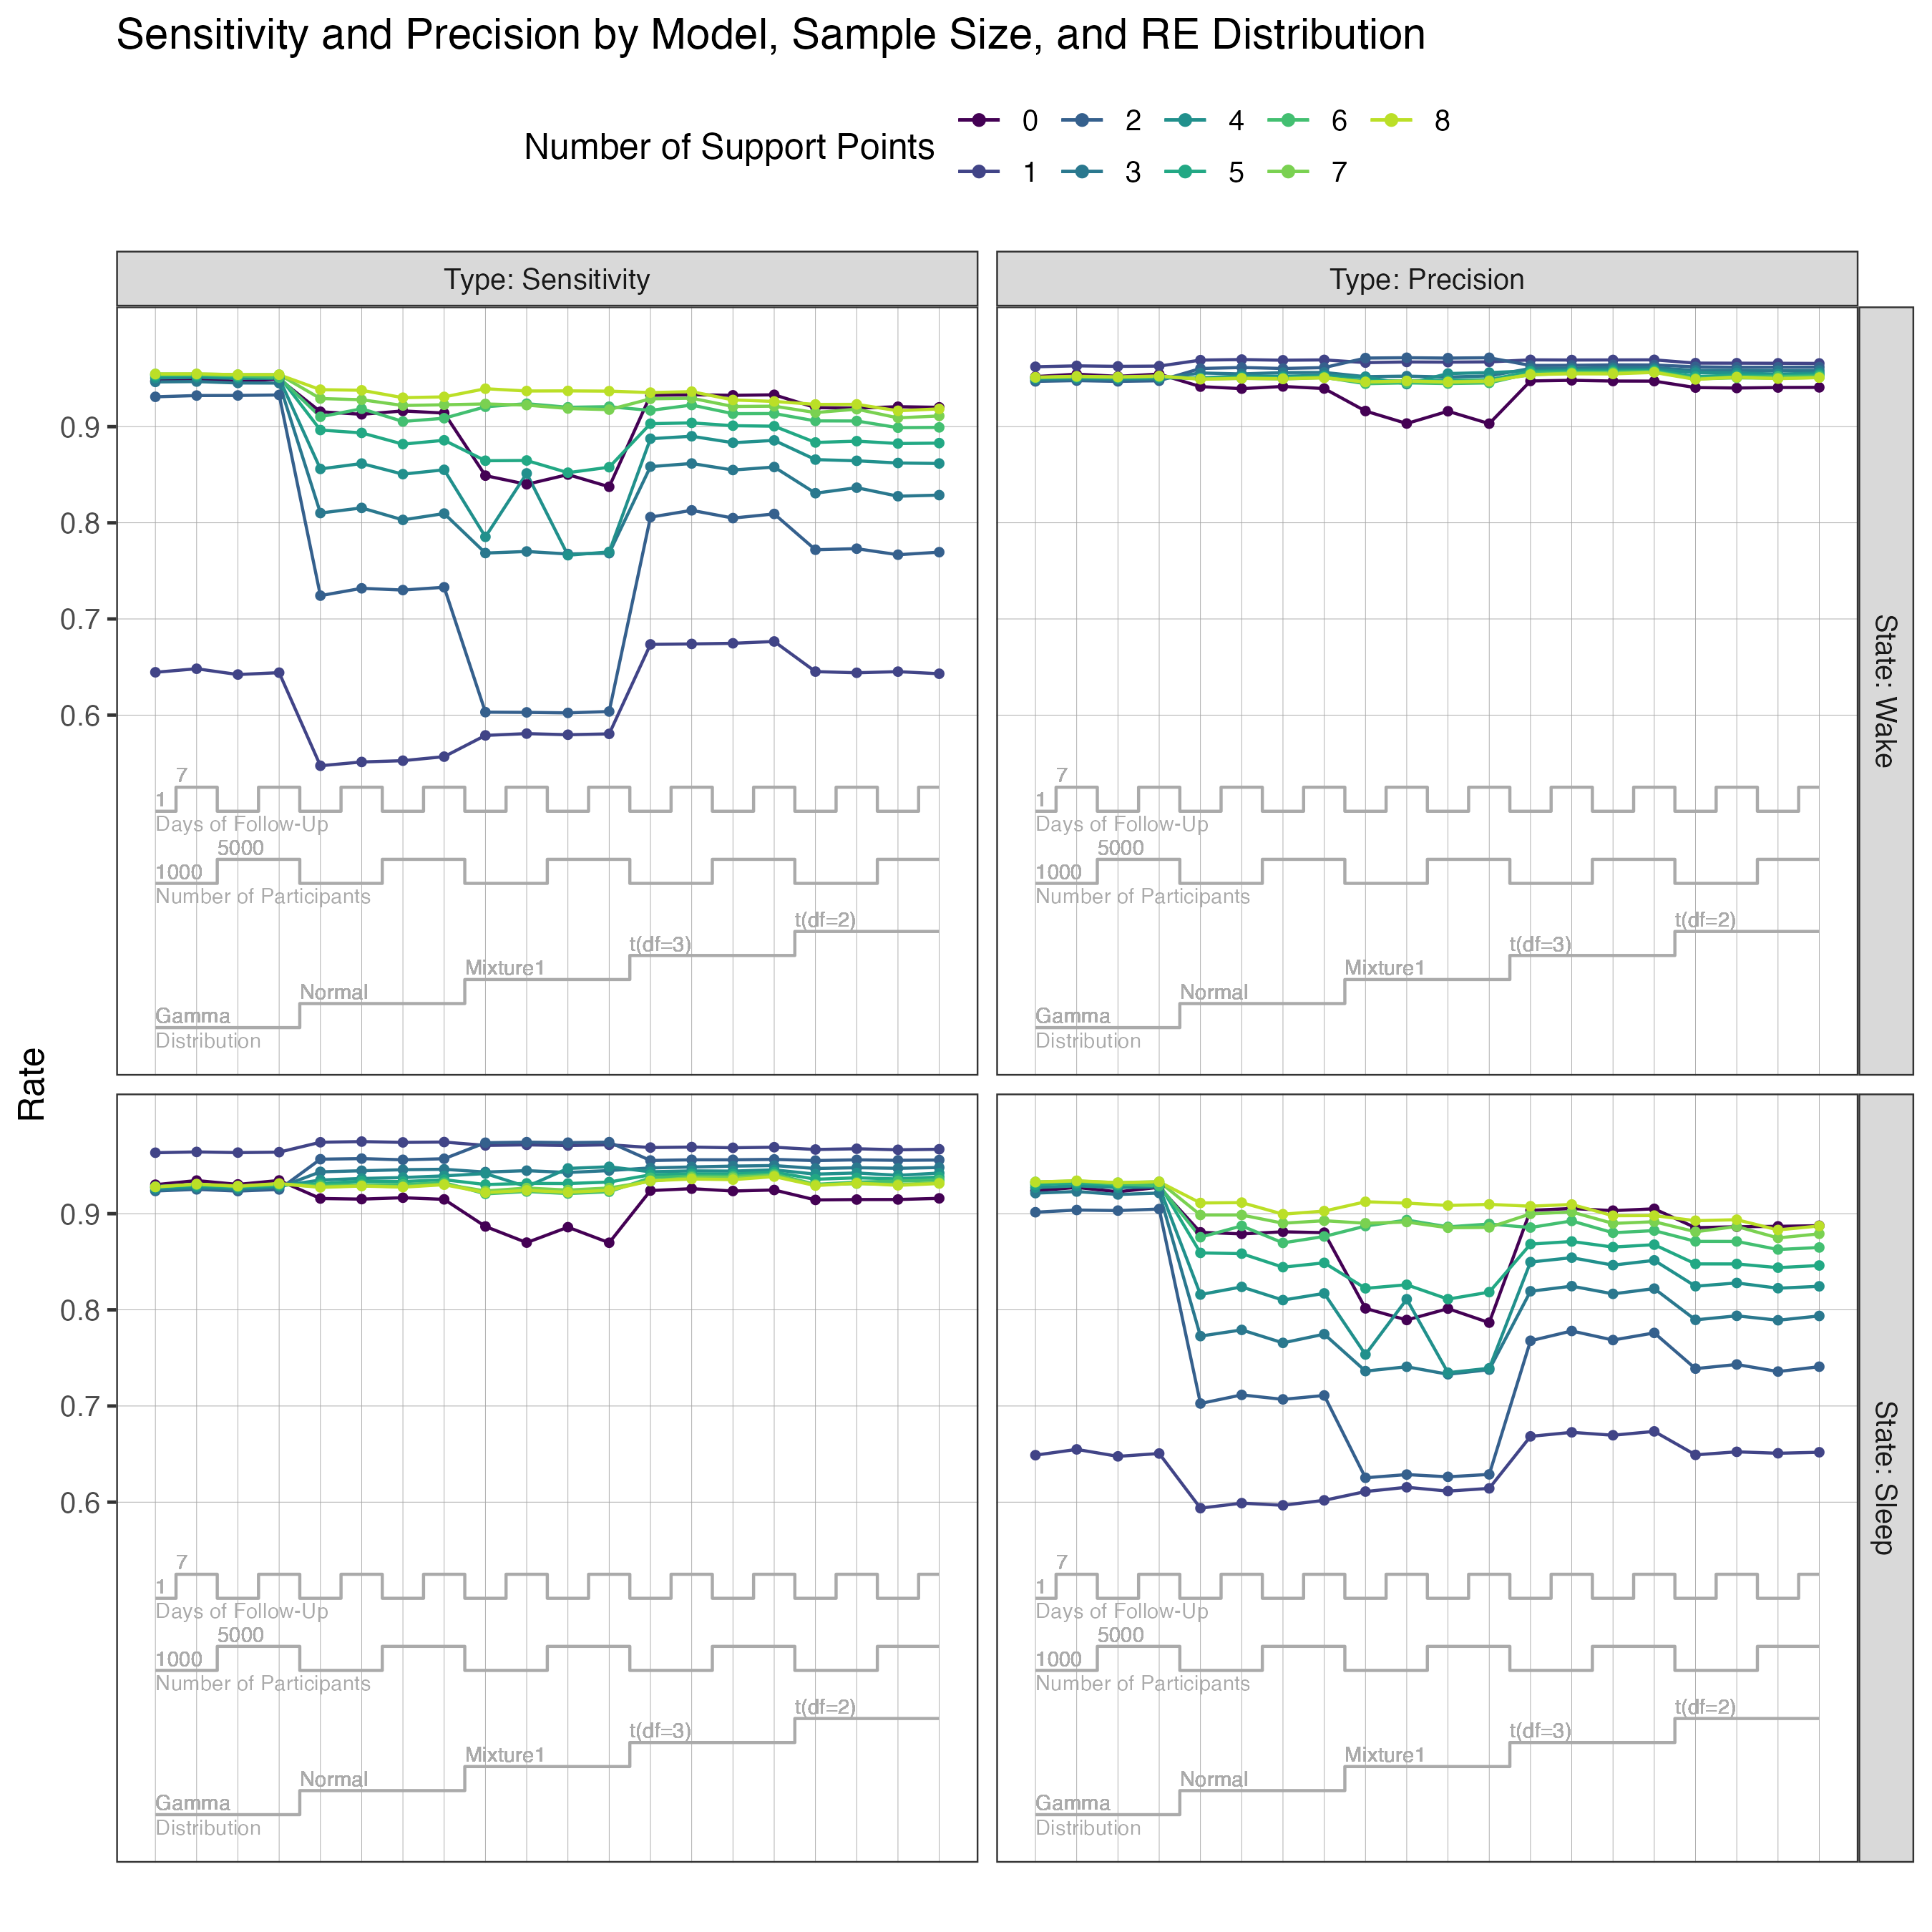
\includegraphics[scale=.65]{Support/NestedLoopSP.png}
\centering
\caption{Nested loop plot of simulation results for 
sensitivity (left column) and precision (right column) 
for wake (top row) and sleep (bottom row). Each point is
 the median of 100 simulations and the color indicates 
 the number of support points. The X axis indicates the 
 simulation settings, which are a combination of days follow-up, 
 number of participants, and RE distribution. Precision may also 
 be referred to as the positive predictive value.}
\label{NL2}
\end{figure}

To get a better understanding of how the method is working we examine the sensitivity and positive predictive value (PPV). Figure \ref{NL2} shows the sensitivity (left column) and PPV (right column) for the wake (top row) and sleep (bottom row) states. Recall that wake sensitivity is the percent of all truly wake states that we accurately predict as wake, and wake PPV is the percent of predicted wake states that are truly wake. FEW SENTENCE ABOUT IND HMM

When we fit a shared HMM and two support point MHMM, we see that although the sleep sensitivity is high, the wake sensitivity is very low. This is because unless the activity for time $t$ is very high, the state at time $t$ is predicted to be sleep. Therefore, we are classifying all low activity wake behavior as sleep. This can be seen by looking at the PPV. The sleep precision is low because we classify truly wake states as sleep. On the other hand, wake precision is very high because although we rarely predict wake, we do so only if we see a high activity measure.

When the number of support points is increased, the wake sensitivity increases, while the sleep sensitivity decreases slightly. This occurs as, although we are better at classifying low activity wake behavior as wake, we also misclassify some sleep activity as wake. This causes wake PPV to decrease and sleep PPV to increase. Overall, total accuracy is increased when the number of support points is increased as we can better classify wake states when we observe low activity measurements. Similar to overall accuracy (figure \ref{NLacc}), the individual HMM preforms similarly to a HMHH with five to eight support points, depending on the simulation settings.


The number of support points needed depends on the spread of the 
underlying continuous RE distribution. When the spread is smaller, 
such as in the gamma simulation, three to four support points are sufficient. 
When the spread is larger, for instance as in the normal distribution, 
five to six support points are necessary. Looking closely at the 100 
simulations for 5000 people with a week of follow up when H is 
the normal distribution we can get a better sense of how increasing 
the number of support points increases overall accuracy. 
This simulation corresponds to the eighth column of points starting 
from the left in figure \ref{NLacc}. 

Figure \ref{CMM} contains information on the cluster mean 
$(\hat{\nu_l})$ in the top row and the mixing proportion 
$(\pi_l)$ in the bottom row. Each gray box indicated the 
total number of support points used in the model and the 
column of the plot is the specific support points starting 
with the first on the left and the last. Each boxplot 
incorporates data from 100 simulations. With one support point 
we have one cluster at around 3.75 and roughly 67\% accuracy. 
With two support points we still have a cluster at around 3.75 
and an additional cluster below 0. This new cluster around 0 is 
responsible for the ability to accurately predict the underlying 
state for sedentary people (i.e. those whose mean wake activity 
is similar to their sleep activity) and increases the overall 
accuracy to 75\%. However with these two support points, we may 
still inaccurately predict the underlying state when we observe 
a mean activity between 0 and 3.75. For instance, if we observe 
a mean activity of 2 for person i, it is unclear which cluster 
person $i$ belongs to. When we use three support points the clusters 
are now at -.75, 2, and 4.5 and can accurately cover a wide range 
of mean wake activities. 

\begin{figure}
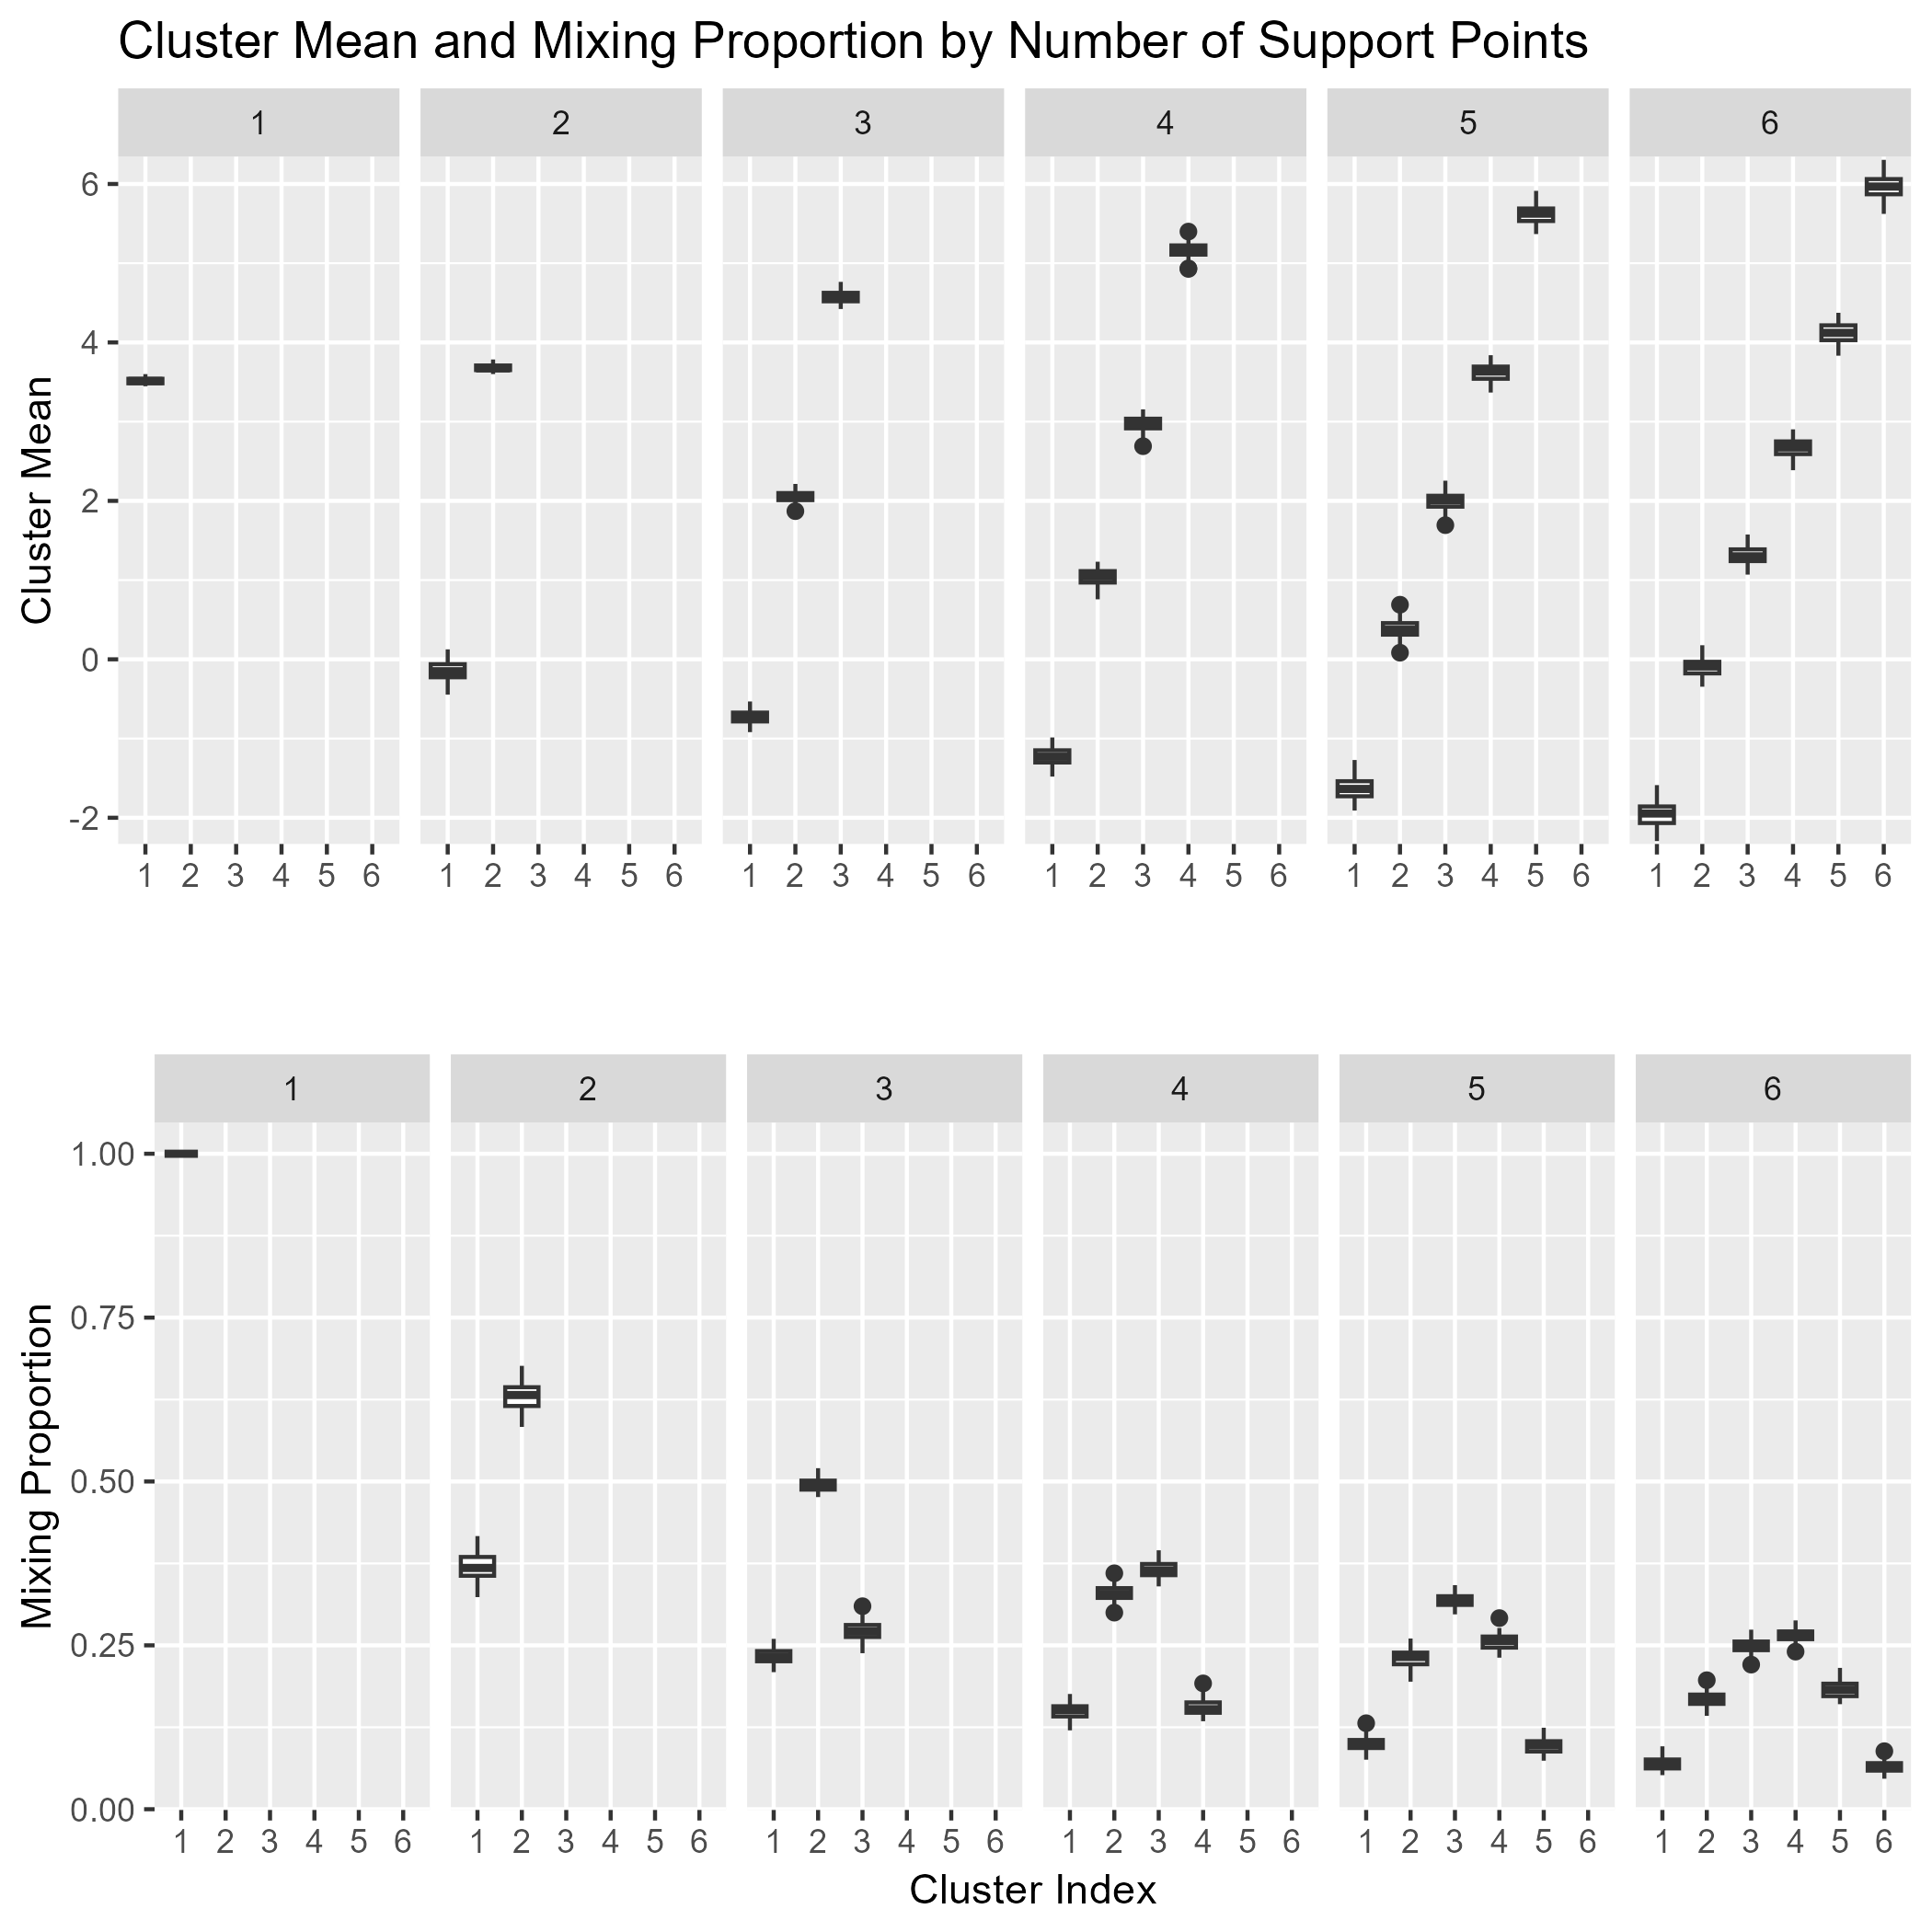
\includegraphics[scale=.48]{Support/clustmeanmix.png}
\centering
\caption{Cluster mean (top row) and mixing proportion (bottom row) 
for number of support points. Each column signifies the number 
of support points starting with one on the left and six on the right. 
Cluster mean represents $\nu_l=\mu_0+r_l$ and the mixing 
proportion is $r_l$. Each boxplot uses data from 100 simulations. }
\label{CMM}
\end{figure}


\subsection{Discussion}\label{SimStudyDiscussion}

It should be noted that the individual HMM is only possible if there are many measurements for each person and drastically increases the number of estimated parameters. In simulations with 96 observations per person, some individual variances were estimated to be zero. Four emission parameters are estimated for the shared HMM. The number of emission parameters for the MHMMs is three plus the number of support points, which ranges from five to 12. For the individual HMM, the number of emission parameter is three plus the number of individuals in the data, which ranges from 1,003 to 5,003

The individual mean activity HMM is extremely flexible and is able to capture minute differences in activity. However, it has a number of key drawbacks. A large number of repeated measurements are needed per person to estimate each mean parameter. It is not clear how prediction would work for a new person without re-estimating the entire model. Finally, the number of parameters scales with the number of people. Despite the much smaller number of parameters, a MHMM either preforms similarly or better than the individual mean activity HMM depending on the number of support points across all simulations. When the underling RE is Gamma or t-distributed (with 2 or 3 df) a MHMM with 8 support points has similar accuracy to the individual HMM. When the RE is Normally distributed the individual HMM is similar to a MHMM with 6 support points. Additionally, MHMMs do not face the same issues as the individual mean activity HMM. MHMMs do not require a large number of repeated measurements per person and are parsimonious in estimated parameters. MHMMs also naturally cluster the data and therefore are very interpretable when focussing on heterogeneity in a population. 

As noted before, there is a trade-off between the number of 
support points and computation time that must be balanced. 
Increasing the number of support points increases the accuracy 
of the state reconstruction, however there are diminishing returns. 
As the necessary computation time roughly scales linearly with 
the number of support points, it is pertinent that we choose enough 
support points to accurately estimate the sequence without 
significant computational burden. Figure \ref{time} is a nested 
loop plot showing the median running time in hours. We see that 
the increasing the number of support points generally increases 
the median running time. Additionally, for all of the simulations 
barring the t distribution with two degrees of freedom, two to 
four support points is sufficient for maximum accuracy as there 
is a steep drop off afterwards. For a t distribution with two 
degrees of freedom it may be beneficial to use six support points, despite the increased time.

\section{Conclusion}

Mixed hidden Markov models are a recent adaptation of HMMs 
which can account for individual level heterogeneity. In this 
paper we have shown that when the data is truly generated with 
a RE in the emissions distribution, a MHMM preforms much better 
than a HMM for state prediction. As the RE distribution is 
estimated using nonparametric density estimation, we have also 
shown that only a small number of support points are needed, 
where the exact number depends on the underlying continuous 
RE distribution. When this distribution has a higher variance, 
more support points are necessary for accurate state estimation. 
Although increasing the number of support points increases 
overall accuracy, it also increases the time needed to fit the model. 
Therefore, a balance must be found between accuracy and 
computation time. We suggest using two to four support points, 
as this provides both high accuracy and shorter running times. 


\begin{figure}
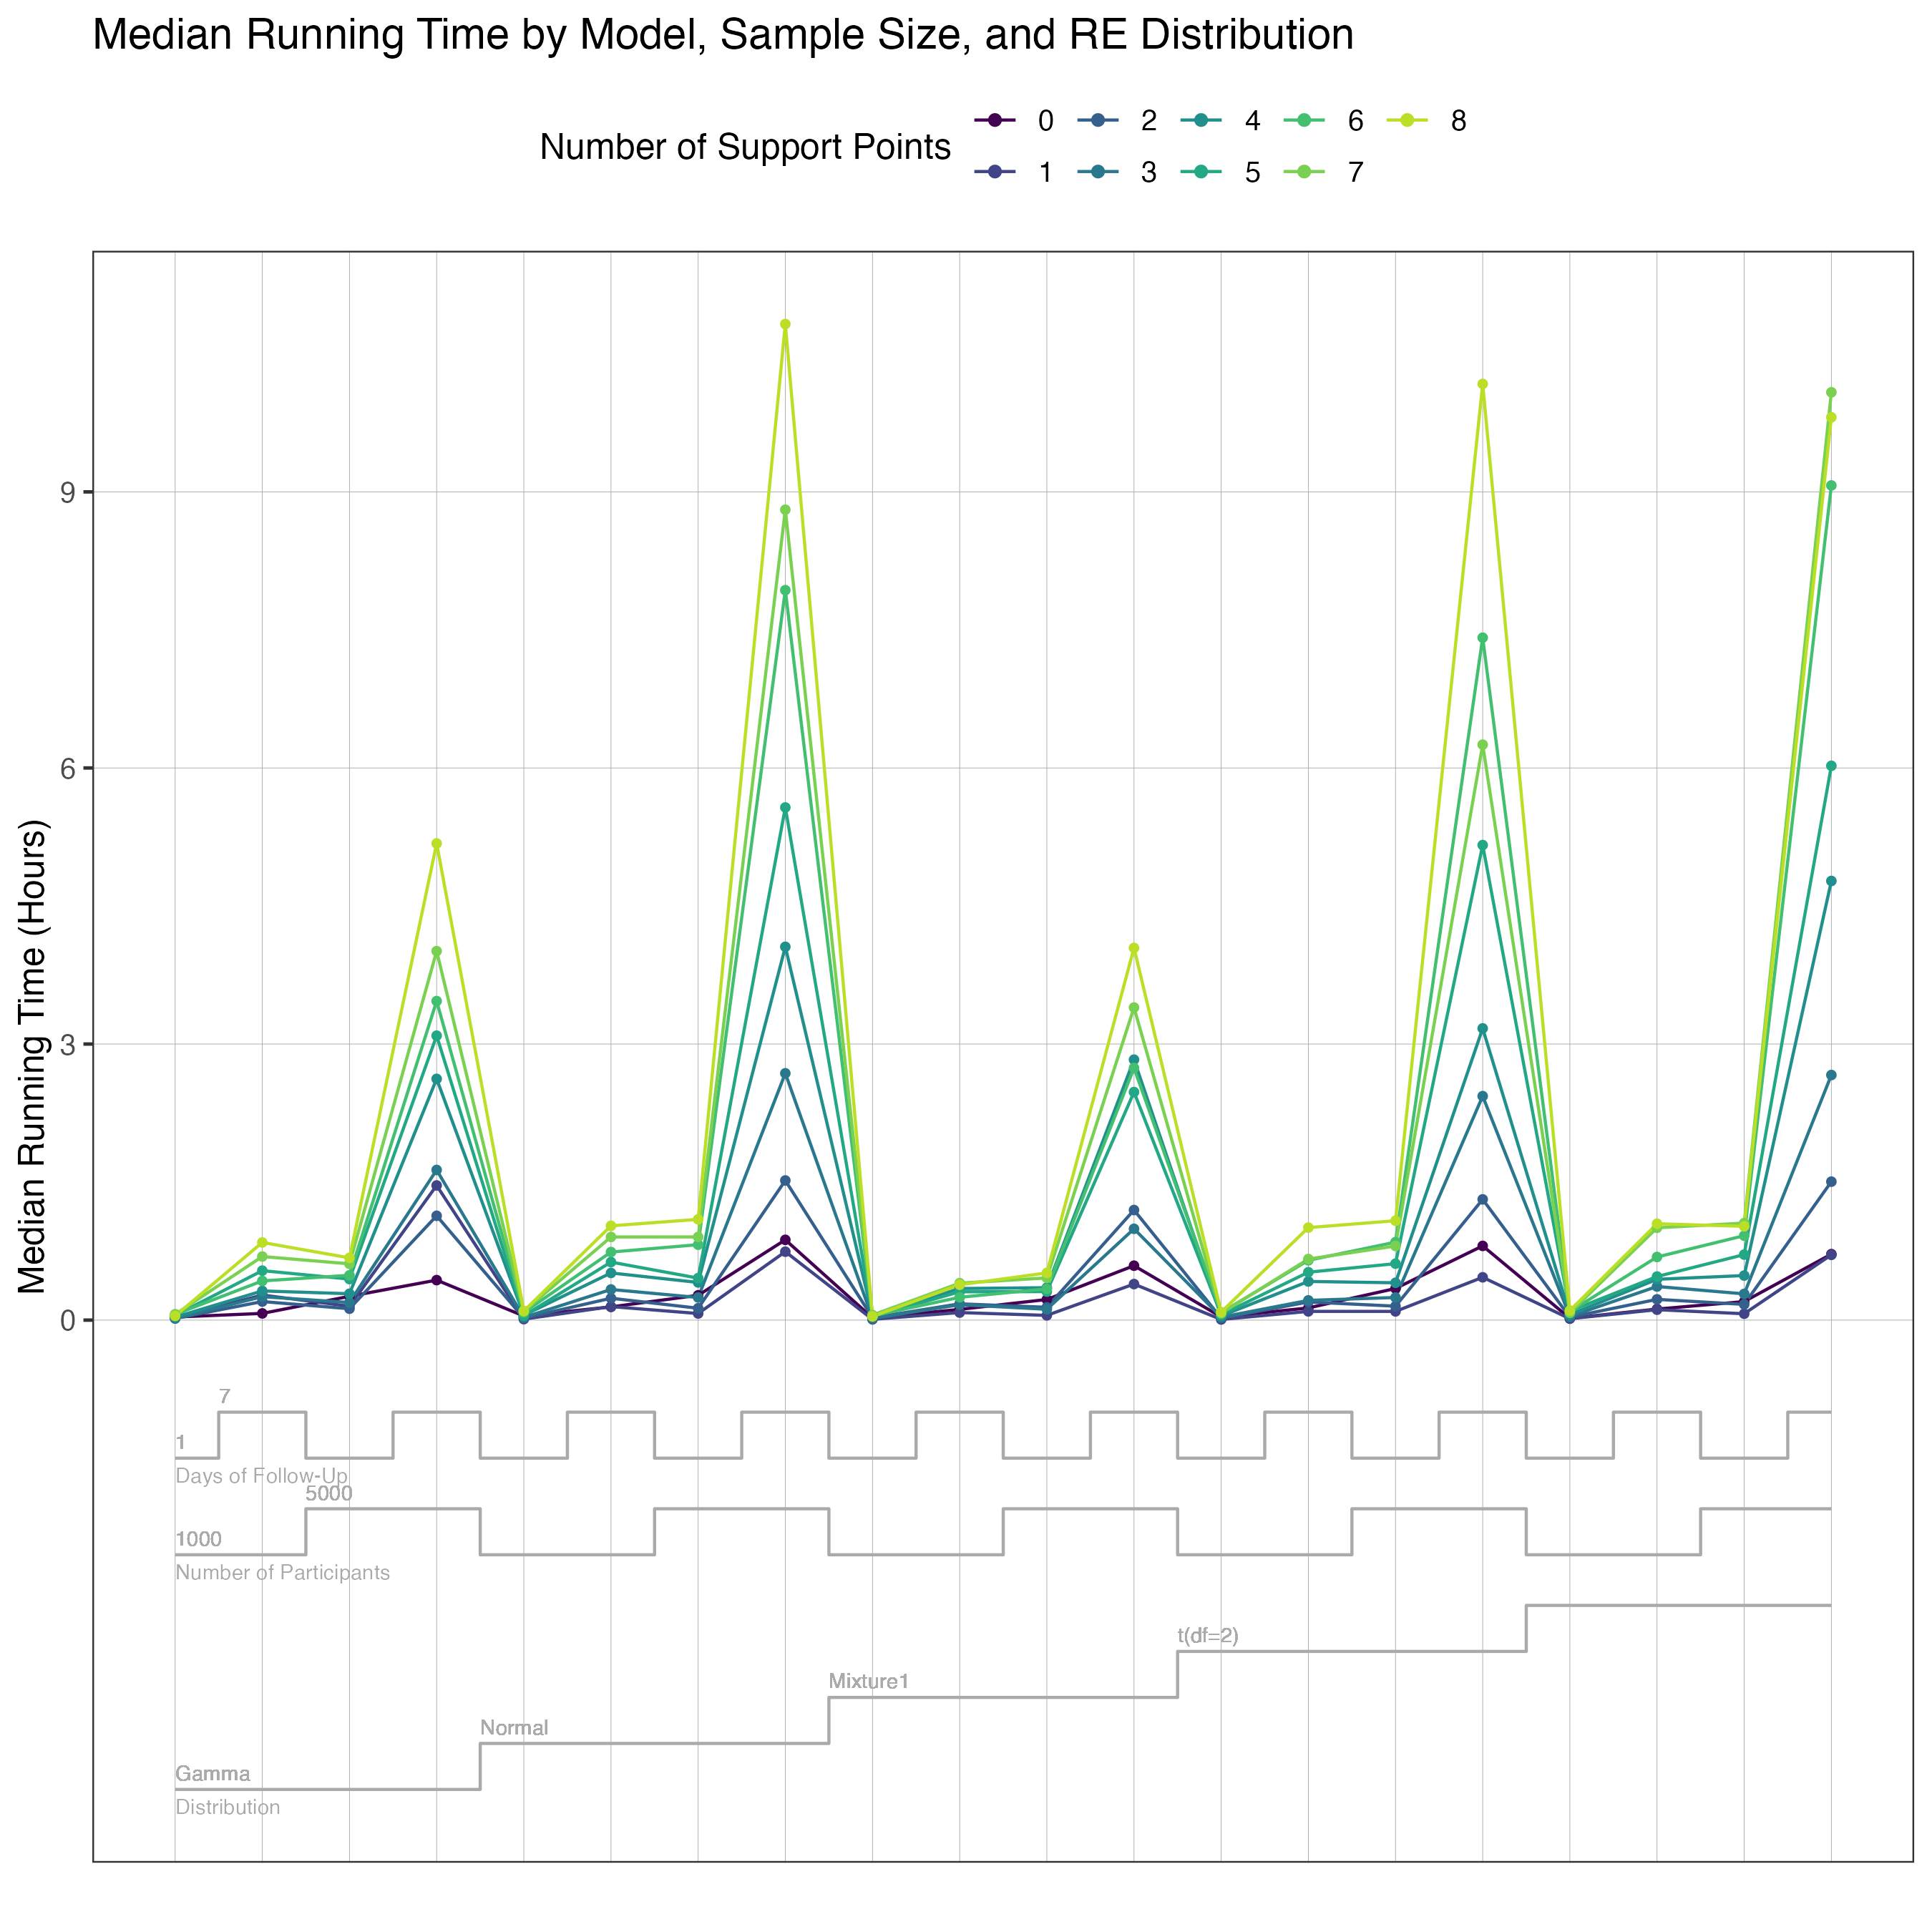
\includegraphics[scale=.55]{Support/NestedLoopCompTime.png}
\centering
\caption{Nested loop plot of simulation results for median 
running time in hours. Each point is the median of 100 simulations 
and the color indicates the number of support points. 
The X axis indicates the simulation settings, which is a 
combination of days follow-up, number of participants, and RE distribution.}
\label{time}
\end{figure}


\bibliographystyle{unsrt}
\bibliography{Support/MHMMbib}

\end{document}
